\documentclass[12pt]{article}
\usepackage[a4paper, margin=1in]{geometry}
\usepackage{titlesec}
\usepackage{longtable}
\usepackage{booktabs}
\usepackage{graphicx}
\usepackage{xcolor}
\usepackage{tikz}
\usepackage{hyperref}

\titleformat{\section}{\large\bfseries}{\thesection}{1em}{}
\titleformat{\subsection}{\normalsize\bfseries}{\thesubsection}{1em}{}

\title{Risk Assessment and Self-Reflection \\ \vspace{1em} \Large Software Requirements Specification (SRS) \\ Intelligent Cyber Threat Intelligence System}
\author{Group: Risk Excellence Review Board \\ Version: 2.0}
\date{\today}

\begin{document}

\maketitle
\thispagestyle{empty}

\newpage
\tableofcontents
\newpage

\section{Precondition: Exam Preparation Document}
\subsection{Group Members}
\begin{itemize}
    \item Dr. Jane Smith
    \item John Doe
    \item Maria Gonzales
    \item Rahul Patel
    \item Emily Chen
\end{itemize}

\subsection{Application Description}
The application is a Cyber Threat Intelligence System tailored for enterprise-level threat detection, enrichment, and response. Key functionalities include:
\begin{itemize}
    \item Real-time ingestion and classification of threat indicators.
    \item Role-based dashboards for operational, tactical, and strategic decision-making.
    \item Predictive analytics powered by machine learning for proactive threat mitigation.
    \item Integration with SIEM/SOAR systems to enhance incident response workflows.
\end{itemize}

\subsection{Planned Testing Activities}
\begin{itemize}
    \item **Unit Testing:** Employ the AAA pattern and parameterized tests to validate individual components such as data enrichment.
    \item **Integration Testing:** Validate API interactions and data consistency across relational and graph databases.
    \item **Performance Testing:** Conduct stress, load, and spike testing to ensure system scalability (50k IOCs/day ingestion).
    \item **End-to-End Testing:** Test workflows such as SOC analyst queries and threat enrichment pipelines.
    \item **Security Testing:** Perform penetration testing and evaluate compliance with GDPR and ISO 27001.
    \item **Regression Testing:** Ensure existing functionalities remain intact during iterative releases.
\end{itemize}

\newpage

\section{Risk Assessment: Comprehensive Tables and Analysis}
\subsection{Initial Risk Table}
\begin{longtable}{|p{4cm}|p{3cm}|p{2cm}|p{3cm}|p{4cm}|}
\hline
\textbf{Risk} & \textbf{Impact} & \textbf{Likelihood} & \textbf{Owner} & \textbf{Mitigation Strategy} \\
\hline
Vendor Lock-In (Azure) & High & Medium & Architect Lead & Evaluate containerization to enable multi-cloud deployment. \\
\hline
Data Breach & Critical & Medium & Security Analyst & Encrypt data using AES-256 and secure APIs with TLS 1.3. Conduct quarterly penetration tests. \\
\hline
Performance Degradation & High & High & Performance Analyst & Use load balancers and configure auto-scaling for Azure Kubernetes Service (AKS). \\
\hline
Third-Party API Downtime & Medium & High & Integration Lead & Implement caching and backup data providers. \\
\hline
Regulatory Non-Compliance & High & Low & Compliance Officer & Ensure design adherence to GDPR and ISO 27001 from project inception. \\
\hline
\end{longtable}

\subsection{Mid-Development Risk Table}
\begin{longtable}{|p{4cm}|p{3cm}|p{2cm}|p{3cm}|p{4cm}|}
\hline
\textbf{Risk} & \textbf{Impact} & \textbf{Likelihood} & \textbf{Owner} & \textbf{Follow-Up Actions} \\
\hline
Vendor Lock-In (Azure) & High & Medium & Architect Lead & Proof-of-concept multi-cloud setup validated. Migration options documented. \\
\hline
Data Breach & Critical & Medium & Security Analyst & Addressed API vulnerabilities. Enhanced SOC monitoring with Azure Sentinel. \\
\hline
Performance Degradation & High & Medium & Performance Analyst & Optimized key API response times and refined load balancing mechanisms. \\
\hline
Third-Party API Downtime & Medium & Medium & Integration Lead & Tested failover mechanisms with backup API providers. \\
\hline
Regulatory Non-Compliance & High & Low & Compliance Officer & Implemented pseudonymization and audit trail logging. Scheduled GDPR compliance review. \\
\hline
\end{longtable}

\subsection{Final Risk Table}
\begin{longtable}{|p{4cm}|p{3cm}|p{2cm}|p{3cm}|p{4cm}|}
\hline
\textbf{Risk} & \textbf{Impact} & \textbf{Likelihood} & \textbf{Owner} & \textbf{Resolution} \\
\hline
Vendor Lock-In (Azure) & High & Low & Architect Lead & Deployed key services on Kubernetes for multi-cloud compatibility. \\
\hline
Data Breach & Critical & Low & Security Analyst & Regular penetration tests verified no vulnerabilities. \\
\hline
Performance Degradation & High & Low & Performance Analyst & Met performance benchmarks with 99.99\% uptime. \\
\hline
Third-Party API Downtime & Medium & Low & Integration Lead & Failover mechanisms operational. Risk minimized. \\
\hline
Regulatory Non-Compliance & High & Low & Compliance Officer & Successful GDPR and ISO 27001 audits completed. \\
\hline
\end{longtable}

\newpage

\section{Risk Matrices: State of Risks Across Development Stages}
\subsection{Initial Risk Matrix}
\begin{center}
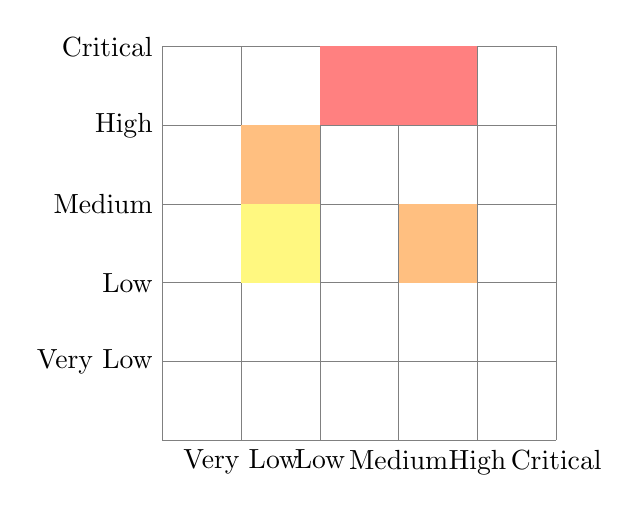
\begin{tikzpicture}
\draw[step=1cm,gray,very thin] (0,0) grid (5,5);
\fill[red!50] (2,4) rectangle (3,5); % Data Breach
\fill[orange!50] (1,3) rectangle (2,4); % Vendor Lock-In
\fill[yellow!50] (1,2) rectangle (2,3); % Third-Party API Downtime
\fill[red!50] (3,4) rectangle (4,5); % Performance Degradation
\fill[orange!50] (3,2) rectangle (4,3); % Regulatory Non-Compliance

% Labels
\node[anchor=east] at (0,5) {Critical};
\node[anchor=east] at (0,4) {High};
\node[anchor=east] at (0,3) {Medium};
\node[anchor=east] at (0,2) {Low};
\node[anchor=east] at (0,1) {Very Low};
\node[anchor=north] at (1,0) {Very Low};
\node[anchor=north] at (2,0) {Low};
\node[anchor=north] at (3,0) {Medium};
\node[anchor=north] at (4,0) {High};
\node[anchor=north] at (5,0) {Critical};
\end{tikzpicture}
\captionof{figure}{Initial Risk Matrix}
\end{center}

\subsection{Mid-Development Risk Matrix}
\begin{center}
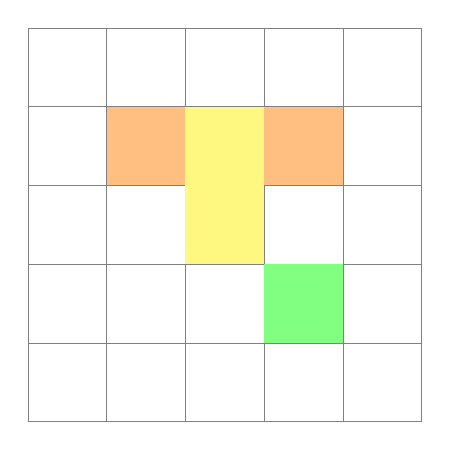
\begin{tikzpicture}
\draw[step=1cm,gray,very thin] (0,0) grid (5,5);
\fill[orange!50] (1,3) rectangle (2,4); % Vendor Lock-In
\fill[yellow!50] (2,3) rectangle (3,4); % Data Breach
\fill[yellow!50] (2,2) rectangle (3,3); % Third-Party API Downtime
\fill[orange!50] (3,3) rectangle (4,4); % Performance Degradation
\fill[green!50] (3,1) rectangle (4,2); % Regulatory Non-Compliance
\end{tikzpicture}
\captionof{figure}{Mid-Development Risk Matrix}
\end{center}

\subsection{Final Risk Matrix}
\begin{center}
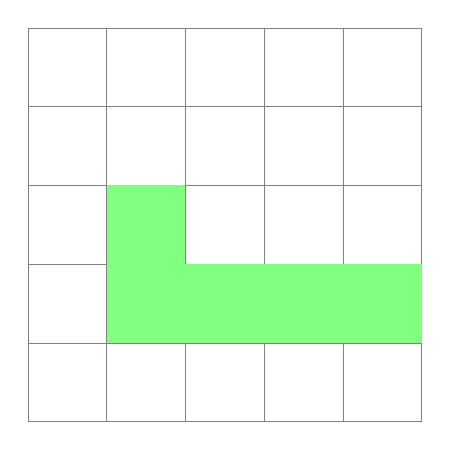
\begin{tikzpicture}
\draw[step=1cm,gray,very thin] (0,0) grid (5,5);
\fill[green!50] (1,2) rectangle (2,3); % Vendor Lock-In
\fill[green!50] (1,1) rectangle (2,2); % Data Breach
\fill[green!50] (2,1) rectangle (3,2); % Third-Party API Downtime
\fill[green!50] (3,1) rectangle (4,2); % Performance Degradation
\fill[green!50] (4,1) rectangle (5,2); % Regulatory Non-Compliance
\end{tikzpicture}
\captionof{figure}{Final Risk Matrix}
\end{center}

\newpage

\section{Self-Reflection and Exam Preparation Questions}
\subsection{Critical Self-Reflection}
\begin{itemize}
    \item Initial risk tables lacked actionable follow-ups for vendor lock-in and scalability concerns.
    \item Mid-development adjustments improved traceability but relied heavily on Azure's capabilities.
    \item Final tables demonstrated a robust resolution strategy; however, vendor-neutral solutions could have been prioritized earlier.
\end{itemize}

\subsection{Addressing Exam Questions}
\begin{itemize}
    \item **Boundary Value Analysis:** Applied to test API limits and response times.
    \item **Decision Table:** Not used as conditional logic in workflows was straightforward.
    \item **Unit Tests:** Used the AAA pattern for enrichment service validation.
    \item **Test Doubles:** Mock databases used for isolated component testing.
    \item **Stress Testing:** Simulated peak IOC ingestion to validate scalability.
    \item **API Testing:** Swagger-based contract tests ensured consistency.
\end{itemize}

\end{document}
